\subsection{Effect of Gravitational waves on objects}

Gravitational waves carry the fluctuations of space along with them. So if they move through an object, since space itself will oscillate, even the object which occupies space will oscillate according to the wave. Thus the shape of object will change periodically.  

\subsubsection{Plus polarized effect}
When a plus polarized wave passes through the object, since such gravitational wave makes space-time oscillate in X and Y axes only. So the points in space along axis will come close during compression and go far during stretching. Thus the object itself will be compressed and stretched along the axes, perpendicular to the direction of propagation of wave.

\subsubsection{Cross polarized effect}
When a cross polarized wave passes through the object, since such gravitational wave makes space-time oscillate along the line which makes an inclination of 45$\degree$ with X and Y axes (i.e. along the line $x=y$ and $x=-y$). So the points in space along those line will come close during compression and go far during stretching. Thus the object itself will be compressed and stretched along those lines, perpendicular to the direction of propagation of wave.
\\

\begin{figure}[h]
    \centering
    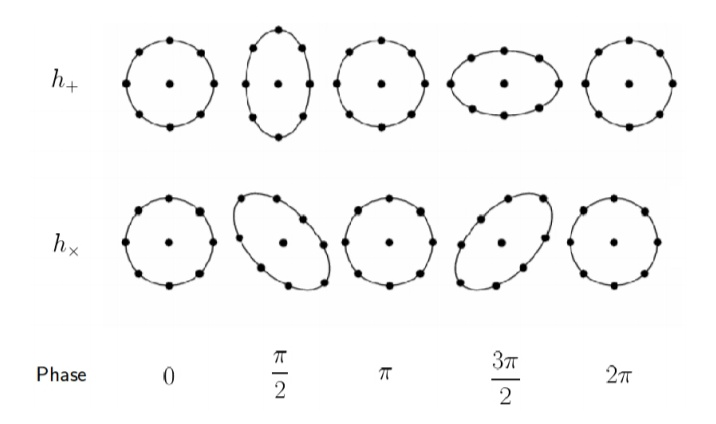
\includegraphics[scale=0.4]{images.tex/effect_of_gw.jpeg}
    \caption{Shape of the object when gravitational wave passes through it when the phase difference of wave changes by $\pi/2$.\\
    \textbf{Source :-} Wavelet graphs for the detection of gravitational waves : application to eccentric binary black holes by Philippe Bacon}
\end{figure}

\begin{figure}[h]
    \centering
    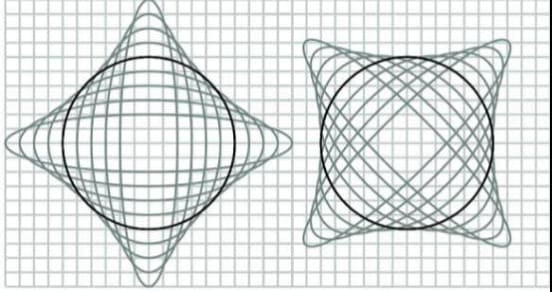
\includegraphics[scale=0.4]{images.tex/polarization.jpeg}
    \caption{Pictorial representation of two Linear polarization of gravitational waves. \\ Source:- \url{https://www.researchgate.net/figure/fig4_228909324}}
\end{figure}

\pagebreak